\section{Simulation}\label{sec:simulation}
Simulations are performed to study how the choice of design parameters like illumination CCT, transmitter SPD, and filter FWHM affect the performance of a multi-colored VLC system. Three transmitting elements with Gaussian emission spectrum at dominant wavelengths of red (627 nm), green (530 nm) and blue (470 nm) are selected. Using these transmitting elements, CCT range of [2500 7000] K is sought. SPD spread within [5 50] nm is considered. \figurename{\ref{fig:LEDSPD}} illustrates normalized SPDs needed to achieve the range of CCTs for transmitting elements with 5 nm spread. Note that for all CCTs, the transmitted radiant flux may vary to achieve a constant target illumination at receiver. 

\begin{figure}[!b]
	\centering
		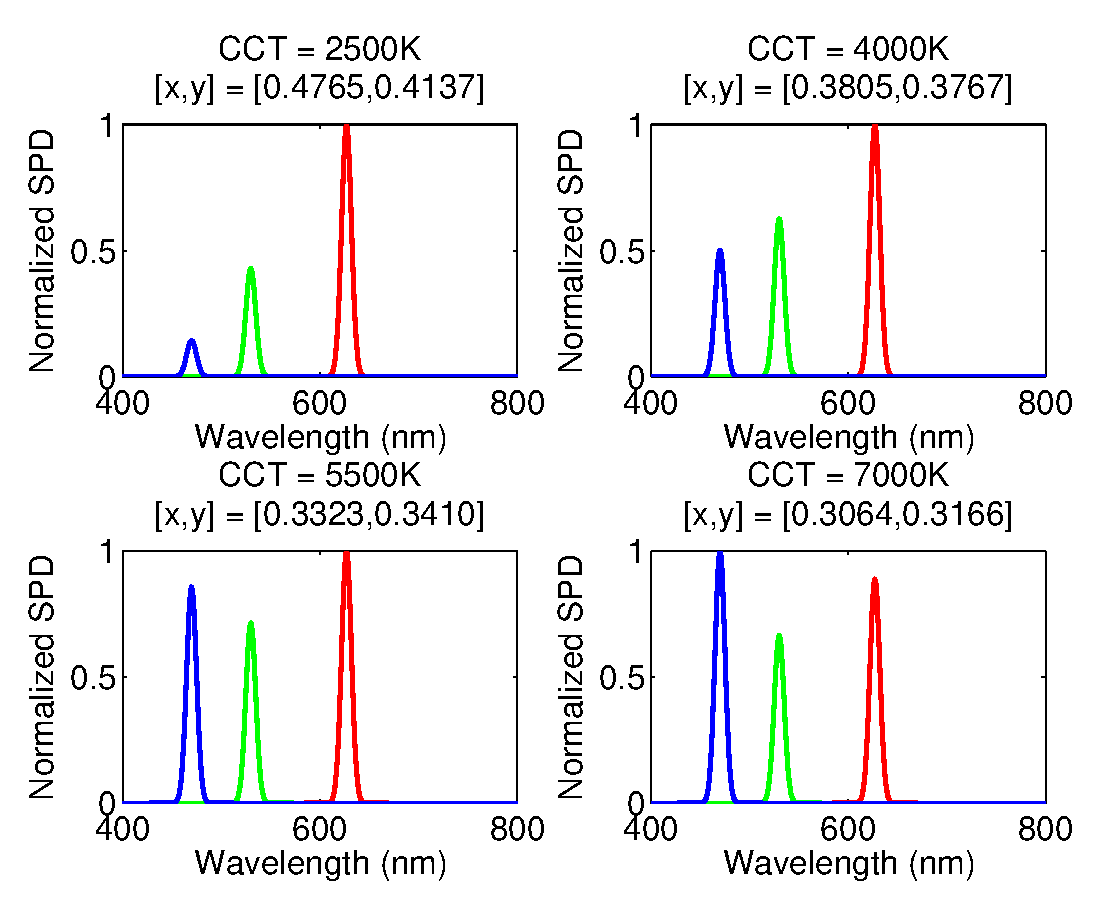
\includegraphics[trim={0.05in 0.05in 0.05in 0.0in}, clip=true, width=2.75in]{img/LEDSPD.eps}
	\caption{Transmitting element normalized spectral power distribution}
	\label{fig:LEDSPD}
\end{figure}

Unique $t_R:t_G:t_B$ ratios are generated after varying the tristimulus values in the range [0 1] in 0.1 unit steps. By substituting these values in Eq.(\ref{eqWhite})-Eq.(\ref{eqChromaticity}), chromaticity coordinates for resulting SPDs are calculated. An initial characterization step generates a pre-populated table consisting of the tristimulus values and corresponding chromaticity coordinates. As the CCT is varied, the chromaticity coordinates are computed as shown in Section \ref{sec:wdm}. From the pre-computed table, the tristimulus values that achieve the closest chromaticity are selected. The SPD is then scaled to achieve target illumination (400 lx) at the receiver that is located at a distance of 2 m from the transmitter. The surface normals of the transmitter and receiver are assumed to be parallel.

\begin{figure}[!t]
	\centering
		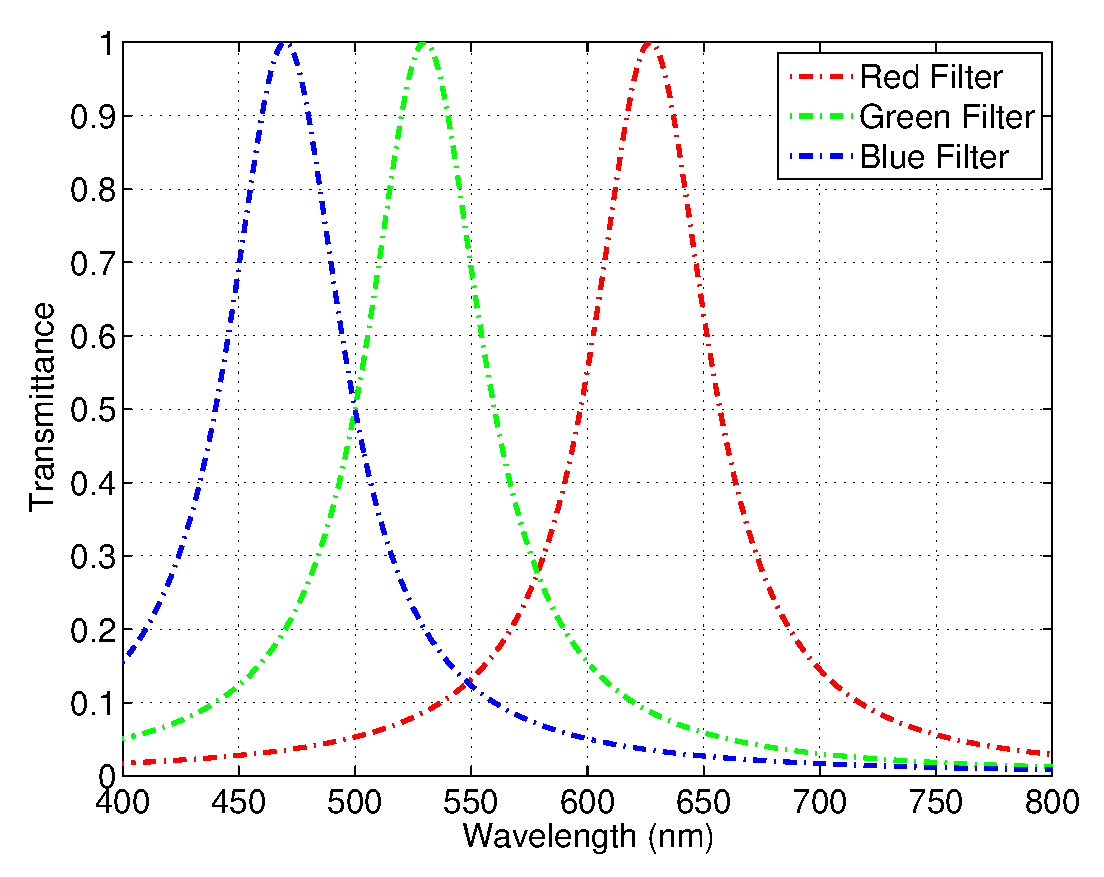
\includegraphics[trim={0.15in 0.05in 0.05in 0.35in}, clip=true, width=2.75in]{img/FiltTr.eps}
	\caption{Filter transmittance for full width at half maximum = 40nm}
	\label{fig:FiltTr}
\end{figure}

Optical filter's passband can be designed to center on the transmitting elements' dominant wavelengths. Optical filters for the simulation are modeled to have Lorentzian transmittance with ideal value $1$ at the dominant red, green and blue wavelengths mentioned above. Filter transmittance as a function of wavelength is illustrated in \figurename{\ref{fig:FiltTr}}. Filter FWHM considered for the analysis lie in [1 250] nm range.

The receiver sensor is assumed to be made of silicon. The assumed quantum efficiencies and responsivity of the sensor taken from source \cite{qeff} is illustrated in \figurename{\ref{fig:RecvResp}}. The responsivity near the blue wavelength is about 0.29 A.W$^{-1}$ and increases steadily to about 0.46 A.W$^{-1}$ near the red before rapidly reducing as the energy of the incident photon approaches the bandgap energy of silicon.

To analyze the system performance, one can start with the system model as described in Eq. (\ref{eqMIMOch}). A random bit stream is then generated. Bits for each link are then using asymmetrically clipped offset and DC-biased optical orthogonal frequency division multiplexing (ACO-OFDM and DCO-OFDM). Details on these optical OFDM techniques can be found in references \cite{car96a,arm06a}. For this simulation, ACO-OFDM and DCO-OFDM are implemented with 64 sub-carriers and 64-QAM and 8-QAM modulation respectively. This ensures that both schemes achieve similar bits/symbol with ACO-OFDM achieving 96 bits/symbol and DCO-OFDM achieving 93 bits/symbol. The DC level on each link is set to ensure the desired CCT is achieved at the 400 lx illumination level. This generates the transmit vector $\vm{X}$. 

\begin{figure}[!b]
	\centering
		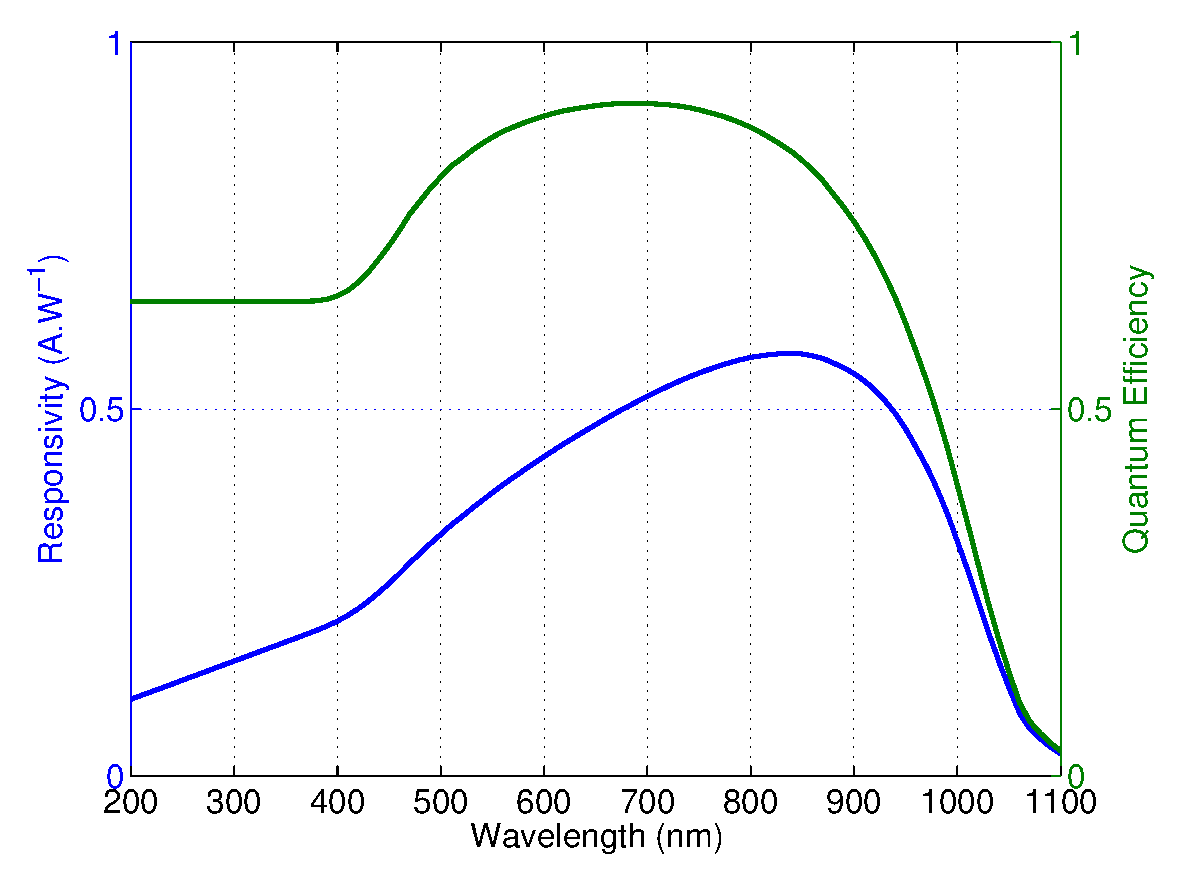
\includegraphics[trim={0.15in 0.05in 0.05in 0.0in}, clip=true, width=2.75in]{img/RecvResp.eps}
	\caption{Receiver quantum efficiency and responsivity \cite{qeff}}
	\label{fig:RecvResp}
\end{figure}

\begin{figure*}[tbph]
\centerline{\subfloat[Most power efficient operation point]{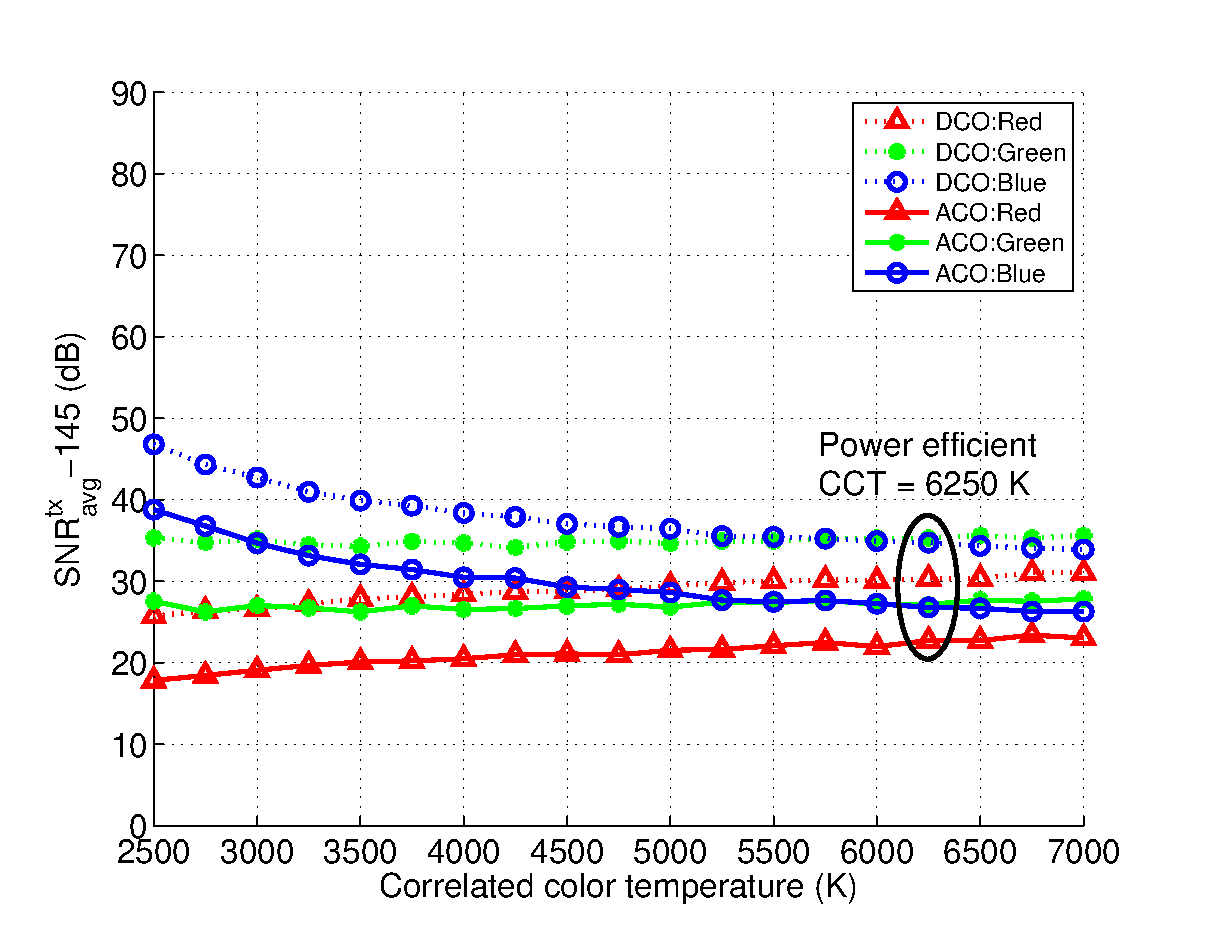
\includegraphics[trim={0.15in 0.05in 0.05in 0.35in}, clip=true, width=2.75in]{img/SNRvsCCT.eps} \label{subfig:SNRvsCCThigh}}
\hfil 
\subfloat[High inter-channel interference]{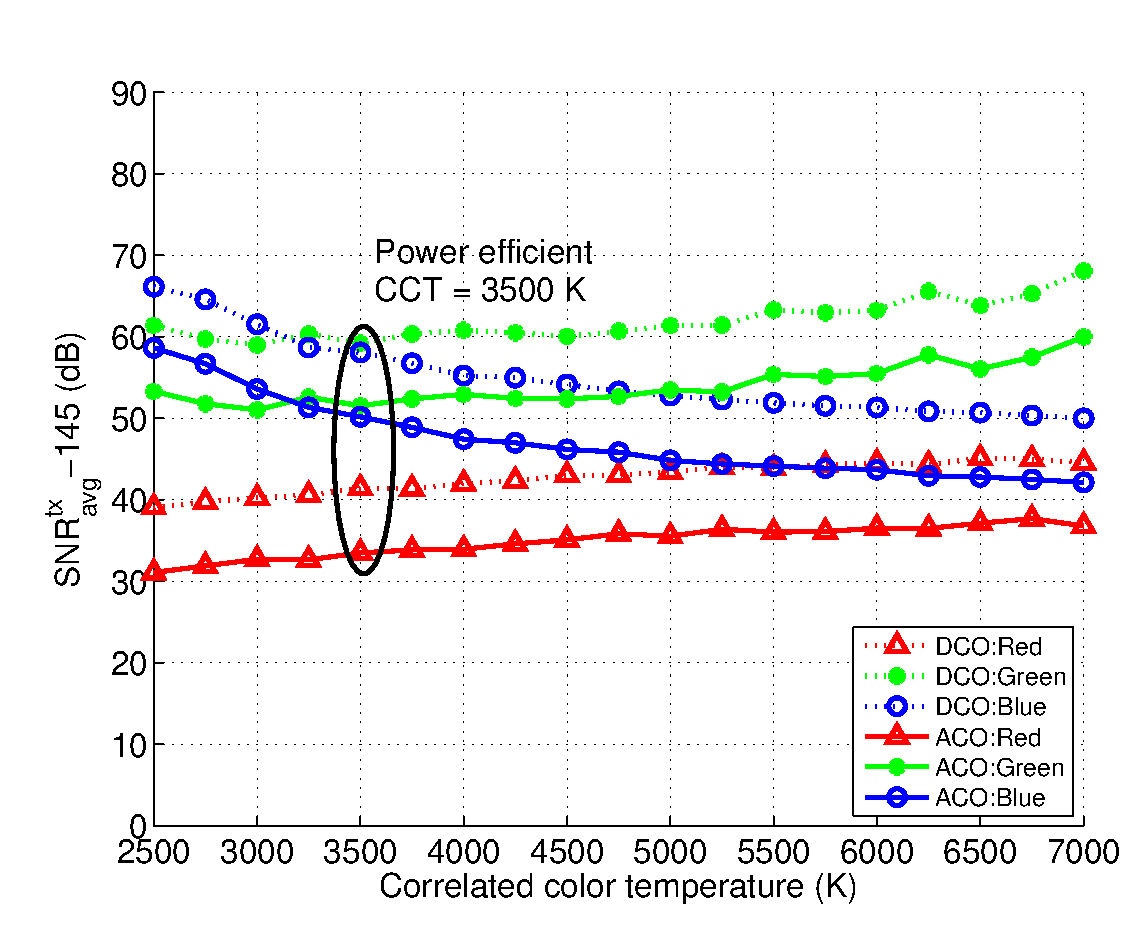
\includegraphics[trim={0.15in 0.05in 0.05in 0.35in}, clip=true, width=2.75in]{img/SNRvsCCT2.eps} \label{subfig:SNRvsCCTlow}}}
\caption{$SNR_{avg}^{tx}$ vs correlated color temperature to achieve BER $\leq 10^{-3}$ \newline(a) Transmitter: $\sigma_r = \sigma_g = \sigma_b = 5$ nm; Filter: $\Gamma_r = \Gamma_g = \Gamma_b = 40$ nm (b) Transmitter: $\sigma_r = \sigma_g = \sigma_b = 50$ nm; Filter: $\Gamma_r = \Gamma_g = \Gamma_b = 250$ nm}
\label{fig:SNRvsCCT}
\end{figure*}
\global\let\figone\relax

Having established $N_{tx} = 3$ transmitting and $N_{rx} = 3$ receiving elements, the $3\times 3$ channel matrix $\vm{H}$ can be computed as in Section \ref{sec:mimo}. Additive white Gaussian noise vector $\vm{W}$ is generated and is then added to the transmitted vector. With the knowledge of the transmitted signal power and by varying the receiver noise, simulations over a range of $SNR_{avg}^{tx}$ are carried out. Vector \vm{Y} then collects the received signal and the added noise and interference. The least squares estimate of the transmitted signal vector is computed as
\begin{equation}
	\label{eqXhat}
	\hat{\vm{X}} = (\vm{H}^{*}\vm{H})^{-1}\vm{H}^{*}\vm{Y}
\end{equation}
An estimate of the transmitted optical OFDM frame for each color is obtained by aggregating least squares estimates of the received signal vectors. Further signal processing on each optical OFDM frame gets an estimate of the transmitted QAM symbol. Decoding the QAM symbols provides an estimate of the transmitted bits. BER is then calculated by comparing the transmit and estimated bit streams.

